% Options for packages loaded elsewhere
% Options for packages loaded elsewhere
\PassOptionsToPackage{unicode}{hyperref}
\PassOptionsToPackage{hyphens}{url}
\PassOptionsToPackage{dvipsnames,svgnames,x11names}{xcolor}
%
\documentclass[
  11pt,
]{article}
\usepackage{xcolor}
\usepackage[top=0.4in,bottom=0.45in,left=0.65in,right=0.65in,includehead,headheight=52pt,headsep=7pt,includefoot,footskip=24pt]{geometry}
\usepackage{amsmath,amssymb}
\setcounter{secnumdepth}{-\maxdimen} % remove section numbering
\usepackage{iftex}
\ifPDFTeX
  \usepackage[T1]{fontenc}
  \usepackage[utf8]{inputenc}
  \usepackage{textcomp} % provide euro and other symbols
\else % if luatex or xetex
  \usepackage{unicode-math} % this also loads fontspec
  \defaultfontfeatures{Scale=MatchLowercase}
  \defaultfontfeatures[\rmfamily]{Ligatures=TeX,Scale=1}
\fi
\usepackage{lmodern}
\ifPDFTeX\else
  % xetex/luatex font selection
\fi
% Use upquote if available, for straight quotes in verbatim environments
\IfFileExists{upquote.sty}{\usepackage{upquote}}{}
\IfFileExists{microtype.sty}{% use microtype if available
  \usepackage[]{microtype}
  \UseMicrotypeSet[protrusion]{basicmath} % disable protrusion for tt fonts
}{}
\makeatletter
\@ifundefined{KOMAClassName}{% if non-KOMA class
  \IfFileExists{parskip.sty}{%
    \usepackage{parskip}
  }{% else
    \setlength{\parindent}{0pt}
    \setlength{\parskip}{6pt plus 2pt minus 1pt}}
}{% if KOMA class
  \KOMAoptions{parskip=half}}
\makeatother
% Make \paragraph and \subparagraph free-standing
\makeatletter
\ifx\paragraph\undefined\else
  \let\oldparagraph\paragraph
  \renewcommand{\paragraph}{
    \@ifstar
      \xxxParagraphStar
      \xxxParagraphNoStar
  }
  \newcommand{\xxxParagraphStar}[1]{\oldparagraph*{#1}\mbox{}}
  \newcommand{\xxxParagraphNoStar}[1]{\oldparagraph{#1}\mbox{}}
\fi
\ifx\subparagraph\undefined\else
  \let\oldsubparagraph\subparagraph
  \renewcommand{\subparagraph}{
    \@ifstar
      \xxxSubParagraphStar
      \xxxSubParagraphNoStar
  }
  \newcommand{\xxxSubParagraphStar}[1]{\oldsubparagraph*{#1}\mbox{}}
  \newcommand{\xxxSubParagraphNoStar}[1]{\oldsubparagraph{#1}\mbox{}}
\fi
\makeatother


\usepackage{longtable,booktabs,array}
\newcounter{none} % for unnumbered tables
\usepackage{calc} % for calculating minipage widths
% Correct order of tables after \paragraph or \subparagraph
\usepackage{etoolbox}
\makeatletter
\patchcmd\longtable{\par}{\if@noskipsec\mbox{}\fi\par}{}{}
\makeatother
% Allow footnotes in longtable head/foot
\IfFileExists{footnotehyper.sty}{\usepackage{footnotehyper}}{\usepackage{footnote}}
\makesavenoteenv{longtable}
\usepackage{graphicx}
\makeatletter
\newsavebox\pandoc@box
\newcommand*\pandocbounded[1]{% scales image to fit in text height/width
  \sbox\pandoc@box{#1}%
  \Gscale@div\@tempa{\textheight}{\dimexpr\ht\pandoc@box+\dp\pandoc@box\relax}%
  \Gscale@div\@tempb{\linewidth}{\wd\pandoc@box}%
  \ifdim\@tempb\p@<\@tempa\p@\let\@tempa\@tempb\fi% select the smaller of both
  \ifdim\@tempa\p@<\p@\scalebox{\@tempa}{\usebox\pandoc@box}%
  \else\usebox{\pandoc@box}%
  \fi%
}
% Set default figure placement to htbp
\def\fps@figure{htbp}
\makeatother





\setlength{\emergencystretch}{3em} % prevent overfull lines

\providecommand{\tightlist}{%
  \setlength{\itemsep}{0pt}\setlength{\parskip}{0pt}}



 


% =====================================================================
%  _style.tex  ·  Design system for EIL research highlights (v8 layout)
%  Edit here to restyle ALL research highlights. Included via the .qmd YAML.
%  Matches the canonical single-column v8 template; the masthead and footer
%  are set per-document via fancyhdr in each .qmd's include-in-header.
% =====================================================================

% ---- Colours (exact hex) --------------------------------------------
\definecolor{ink}{HTML}{1D2620}        % title, masthead rule
\definecolor{body}{HTML}{33352C}       % main body paragraphs
\definecolor{accentred}{HTML}{641111}  % RESEARCH HIGHLIGHT label, links, section heads, fig title
\definecolor{boxred}{HTML}{8C2826}     % Bottom Line box fill
\definecolor{boxtext}{HTML}{EEF1EA}    % Bottom Line body text (off-white)
\definecolor{muted}{HTML}{50534A}      % figure source line
\definecolor{cite}{HTML}{6E6D61}       % citation line
\definecolor{faint}{HTML}{9A978A}      % footer
\definecolor{warmrule}{HTML}{D8D2C2}   % thin warm-grey dividers
\definecolor{paper}{HTML}{FAF8F1}      % warm page background

% \pagecolor{paper}                    % uncomment for warm off-white background

% ---- Fonts (Source Sans 3 / Source Serif 4) -------------------------
\usepackage[T1]{fontenc}
\usepackage[default]{sourcesanspro}
\usepackage{sourceserifpro}
\renewcommand{\familydefault}{\sfdefault}

% ---- Page -----------------------------------------------------------
\pagestyle{empty}
\setlength{\parindent}{0pt}
\setlength{\parskip}{2pt}
% Default body size/colour. The .qmd overrides this to 10.5/13.5pt.
\AtBeginDocument{\color{body}\fontsize{9.4pt}{13.6pt}\selectfont}

% ---- Packages -------------------------------------------------------
\usepackage{microtype}
\usepackage{soul}
\setul{2pt}{.5pt}
\usepackage{tcolorbox}
\tcbuselibrary{skins}
\usepackage[colorlinks=true, urlcolor=accentred, linkcolor=accentred, pdfborder={0 0 0}]{hyperref}

% =====================================================================
%  MACROS
% =====================================================================

% --- Title + citation (citation has a thin warm divider beneath) ------
\newcommand{\brieftitle}[1]{%
  {\color{ink}\fontsize{18pt}{19.5pt}\selectfont\bfseries\textls[-12]{#1}\par}\vspace{3pt}}
\newcommand{\briefcitation}[1]{%
  {\color{cite}\fontsize{9.4pt}{12pt}\selectfont #1\par}\vspace{3pt}%
  \noindent\textcolor{warmrule}{\rule{\linewidth}{0.7pt}}}

% --- Section heads (uppercase, maroon) -------------------------------
\newcommand{\sectionhead}[1]{%
  \vspace{2pt}{\color{accentred}\bfseries\fontsize{9.75pt}{12pt}\selectfont
  \textls[20]{\MakeUppercase{#1}}\par}\vspace{1pt}}

% --- Sub-heads (small uppercase) -------------------------------------
% Legacy — the retired Takeaways block used these. Kept in the brand
% maroon so older highlights that call \subhead still compile.
\newcommand{\subhead}[1]{%
  {\color{accentred}\bfseries\fontsize{8.25pt}{10pt}\selectfont
  \textls[50]{\MakeUppercase{#1}}\par}\vspace{2pt}}

% --- Figure title + source line --------------------------------------
\newcommand{\figtitle}[2]{%
  {\bfseries\color{accentred}\fontsize{7.1pt}{9pt}\selectfont\textls[40]{\MakeUppercase{#1}}}\par%
  {\color{muted}\fontsize{7.1pt}{9pt}\selectfont #2}\par\vspace{4pt}}

% =====================================================================
%  COLOURED BOXES
% =====================================================================

% --- Bottom Line box (border-radius 6px -> arc=4pt) ------------------
\newtcolorbox{bottomline}{%
  enhanced, arc=4pt, outer arc=4pt, boxrule=0pt,
  colback=boxred, coltext=boxtext,
  left=7pt, right=7pt, top=7pt, bottom=7pt,
  before upper={\fontsize{9.4pt}{13.6pt}\selectfont}}

% --- Info box (contact + full citation; centered, thin faint border) --
% Superseded by the moreinfo environment below; kept so older highlights
% still compile. Faint text at footer size. Wrap any link as
% \href{url}{\color{faint}\underline{text}} so it inherits the faint
% colour instead of the global accent link colour.
\newtcolorbox{infobox}{%
  enhanced, width=0.9\linewidth, center, arc=4pt, outer arc=4pt,
  boxrule=0.5pt, colframe=faint, colback=white, coltext=faint,
  left=9pt, right=9pt, top=7pt, bottom=7pt,
  before upper={\fontsize{7.4pt}{9.5pt}\selectfont}}

% =====================================================================
%  CLOSING BLOCK
% =====================================================================

% --- For more information (full width; rule above, no box) ------------
% Four paragraphs: contact line, full citation, author affiliations
% (one bold-lead sentence each), then the EIL boilerplate. Wrap any link as
% \href{url}{\color{cite}\underline{text}} so it inherits the block's
% grey instead of the global accent link colour.
\newenvironment{moreinfo}{%
  \par\vspace{12pt}%
  \noindent\textcolor{warmrule}{\rule{\linewidth}{0.7pt}}\par
  \vspace{7pt}%
  {\color{ink}\bfseries\fontsize{8.25pt}{10pt}\selectfont
   \textls[50]{\MakeUppercase{For more information}}\par}\vspace{4pt}%
  \color{cite}\fontsize{8.4pt}{11.5pt}\selectfont
  \setlength{\parskip}{5pt}%
}{\par}
% --- Background wrap figure ---
\usepackage{wrapfig}
% --- Running masthead + footer (logo, label, rule, page number) ---
\usepackage{fancyhdr}
\renewcommand{\headrulewidth}{0pt}
\renewcommand{\footrulewidth}{0pt}
\fancypagestyle{brief}{%
  \fancyhf{}%
  \fancyhead[L]{%
    \begin{minipage}[c]{0.62\textwidth}\raggedright\color{ink}\includegraphics[height=0.45in]{../../../../formats/logos/eil-logo-maroon.png}\end{minipage}\hfill%
    \begin{minipage}[c]{0.36\textwidth}\raggedleft\fontsize{8.25pt}{10pt}\selectfont\bfseries\color{accentred}\textls[200]{\MakeUppercase{Research Highlight}}\end{minipage}%
    \par\vspace{2pt}%
    \noindent\textcolor{ink}{\rule{\textwidth}{2.2pt}}%
  }%
  \fancyfoot[C]{%
    \color{warmrule}\rule{\textwidth}{0.7pt}\par\vspace{3pt}%
    \hbox to\textwidth{%
      \color{faint}\fontsize{7.4pt}{9pt}\selectfont
      For full paper:\hspace{0.4em}\href{https://www.nber.org/papers/w35675}{\color{faint}\underline{\textls[40]{nber.org/papers/w35675}}}%
      \hfill
      Page \thepage%
    }%
  }%
}
\pagestyle{brief}
\makeatletter
\@ifpackageloaded{caption}{}{\usepackage{caption}}
\AtBeginDocument{%
\ifdefined\contentsname
  \renewcommand*\contentsname{Table of contents}
\else
  \newcommand\contentsname{Table of contents}
\fi
\ifdefined\listfigurename
  \renewcommand*\listfigurename{List of Figures}
\else
  \newcommand\listfigurename{List of Figures}
\fi
\ifdefined\listtablename
  \renewcommand*\listtablename{List of Tables}
\else
  \newcommand\listtablename{List of Tables}
\fi
\ifdefined\figurename
  \renewcommand*\figurename{Figure}
\else
  \newcommand\figurename{Figure}
\fi
\ifdefined\tablename
  \renewcommand*\tablename{Table}
\else
  \newcommand\tablename{Table}
\fi
}
\@ifpackageloaded{float}{}{\usepackage{float}}
\floatstyle{ruled}
\@ifundefined{c@chapter}{\newfloat{codelisting}{h}{lop}}{\newfloat{codelisting}{h}{lop}[chapter]}
\floatname{codelisting}{Listing}
\newcommand*\listoflistings{\listof{codelisting}{List of Listings}}
\makeatother
\makeatletter
\makeatother
\makeatletter
\@ifpackageloaded{caption}{}{\usepackage{caption}}
\@ifpackageloaded{subcaption}{}{\usepackage{subcaption}}
\makeatother
\usepackage{bookmark}
\IfFileExists{xurl.sty}{\usepackage{xurl}}{} % add URL line breaks if available
\urlstyle{same}
\hypersetup{
  colorlinks=true,
  linkcolor={blue},
  filecolor={Maroon},
  citecolor={Blue},
  urlcolor={Blue},
  pdfcreator={LaTeX via pandoc}}


\author{}
\date{}
\begin{document}


% ---------------------------------------------------------------------
% TITLE + CITATION  (masthead repeats in the page header)
% ---------------------------------------------------------------------
{\raggedright\brieftitle{The burden of losing a home to wildfire: income falls for years \mbox{afterward}}}
\briefcitation{Lessons from ``The Distribution and Consequences of Natural Disasters: Evidence from U.S. Wildfire Victims'' by Patrick Baylis, Judson Boomhower, Jonathan Colmer, and John Voorheis, NBER Working Paper, 2026.}

\vspace{-2pt}

% override body font size for this document
\fontsize{10.5pt}{13.5pt}\selectfont

% ---------------------------------------------------------------------
% BOTTOM LINE  (~40–50 words)
% ---------------------------------------------------------------------
\begin{bottomline}
{\fontsize{11pt}{15pt}\selectfont
New research studying around 150 major U.S. wildfires over two decades shows that \textbf{when a wildfire destroys a home, occupants don't just lose the structure --- they lose income too, for years afterward}.
}
\end{bottomline}

\vspace{6pt}

% ---------------------------------------------------------------------
% BACKGROUND  (~2 paragraphs)
% ---------------------------------------------------------------------
\sectionhead{Background}
% Photo: Mike Newbry, via Unsplash (unsplash.com/photos/DwtX9mMHBJ0).
% Unsplash License — commercial use permitted, attribution not required but given.
% wildfire-newbry.jpg is a 1900px working copy; -original.jpg is the 6000px download.
\begin{wrapfigure}{r}{3.25in}
  \vspace{-\intextsep}
  \centering
  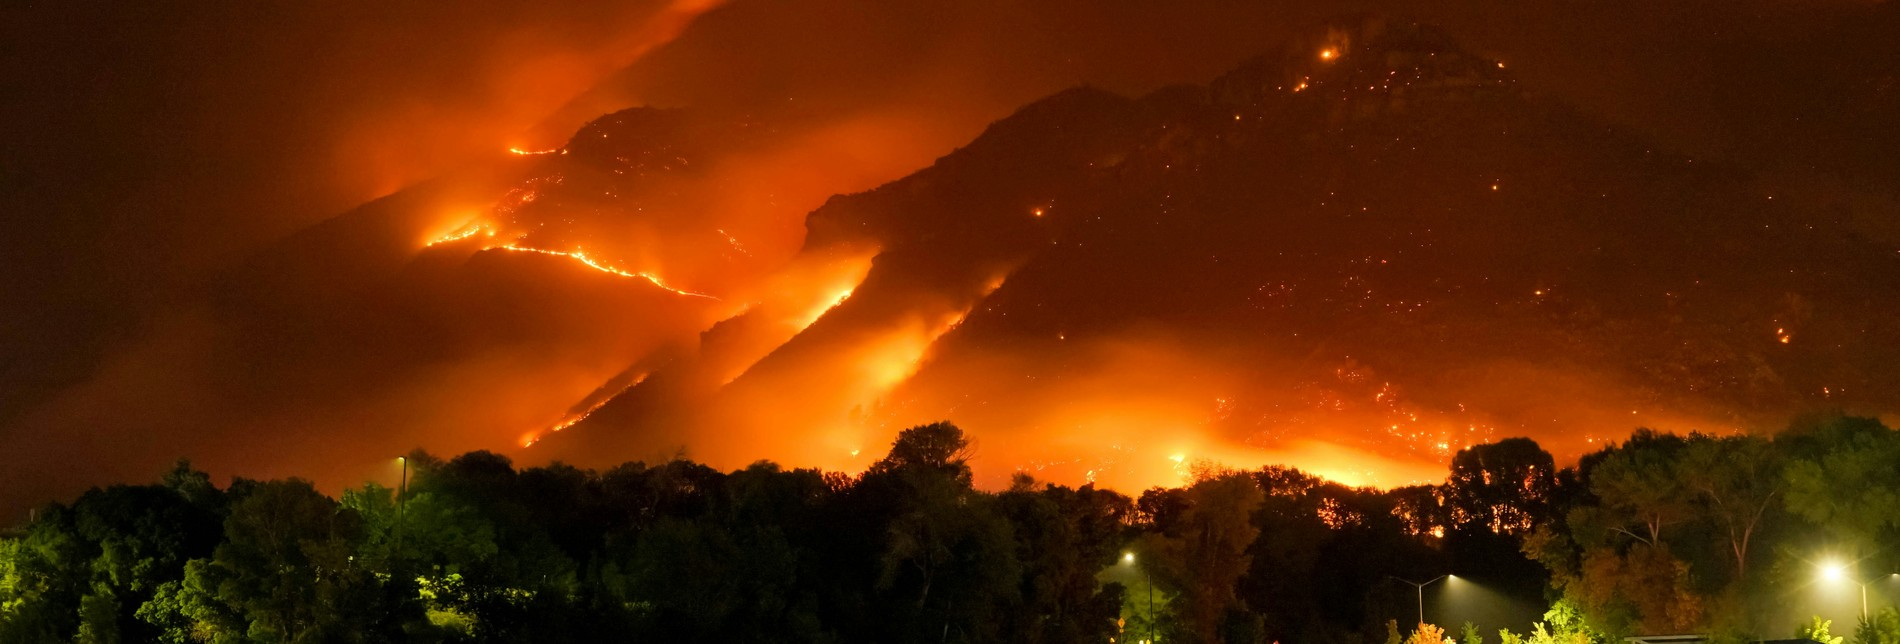
\includegraphics[width=3.1in]{wildfire-newbry.jpg}
  \par\vspace{3pt}
  {\color{faint}\fontsize{7.1pt}{9.5pt}\selectfont \textit{Photo:} Mike Newbry / Unsplash\par}
\end{wrapfigure}
\hyphenpenalty=10000 \exhyphenpenalty=10000
\noindent Global economic losses from natural catastrophes totaled \$320 billion in 2024. This figure helps highlight how important this issue is, but doesn't provide enough information for action to be taken. \textbf{Costs fall unevenly across people and places, which is essential to understand for effective responses.} Destructive wildfires have grown far more common over the past decade, and three forces are expected to push that number higher: a warming climate, more building in fire-prone places, and the dry brush and dead trees that have piled up after decades of fire suppression. Responding well means knowing what these fires cost and who pays.

\noindent Baylis et al.\ studied around 150 major wildfires in five western states between 2003 and 2022, representing more than 7 in 10 of all U.S. homes destroyed by wildfire in that period. They paired official post-fire damage inspections of every structure inside each fire perimeter with tax and Census records to track affected people and their incomes. \textbf{The structural status for every home in each fire's path is matched to the income of the people who lived there, providing an incredibly detailed view of the distributional consequences of wildfires.}
\hyphenpenalty=50 \exhyphenpenalty=50

\vspace{6pt}

% ---------------------------------------------------------------------
% WHO IS IN THE FIRE'S PATH + THE WITHIN-FIRE INCOME GAP
% (merged from two sections when condensing v2 to two pages)
% ---------------------------------------------------------------------
\sectionhead{Lower-income homes burned more often, even on the same street}
\noindent The people in the fires' paths earned more than the U.S. population on average and were more likely to be white, reflecting where wildfires are most prevalent --- the western U.S., many of them in California. However, within any single fire, the people who lost homes earned less than their surviving neighbors: \textbf{occupants of destroyed homes earned \$132,700 on average before the fire, against \$219,800 for occupants of homes that survived the same fires.} A quarter of those who lost a home earned under \$42,000.

\vspace{6pt}

% ---------------------------------------------------------------------
% THE HEADLINE RESULT  (+ figure)
% ---------------------------------------------------------------------
\sectionhead{Income fell only for those who lost a home}
\noindent To measure the costs of the fire outside of home reconstruction, the researchers compared those who did and those who didn't lose a home against people living just outside the perimeter, all in the same job market and same year. All three groups' incomes had moved together for years beforehand, allowing researchers to assume that if those who lost a home had not been affected by the fire, their incomes would have followed the same trajectory as the other groups. However, \textbf{households whose homes were destroyed earned less than their neighbors for three years running, about 11\% less at the low point in the second year, recovering by the fourth}. Added up, the shortfall comes to 30\% of a single year's pre-fire income, roughly \$38,000, while \textbf{households whose homes survived showed no decline in income}.

% figure floats to the top of the next page so the body text can fill
% page 1 instead of leaving a gap where the block wouldn't fit
\begin{figure}[t]
\centering
\begin{minipage}{0.66\linewidth}
\figtitle{The wildfire's effect on income, year by year}{Source: Baylis, Boomhower, Colmer \& Voorheis (2026), Fig.\ 4a.}
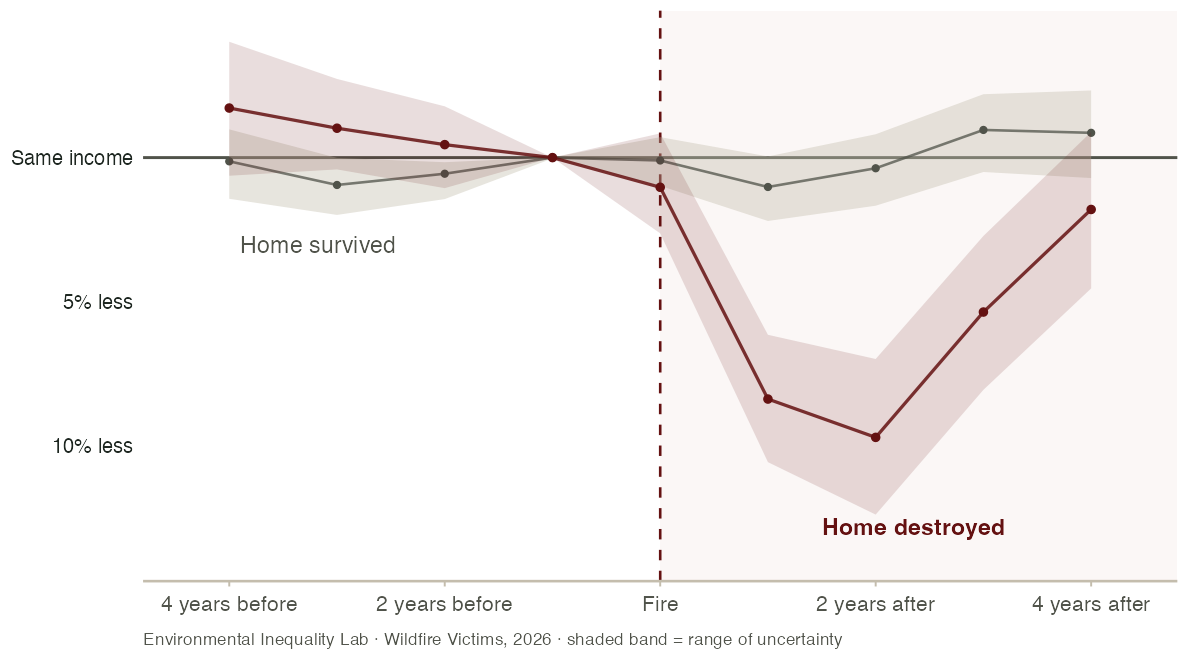
\includegraphics[width=\linewidth]{../../data-viz/figures/fig1-income-by-damage.png}
\par\vspace{3pt}
{\color{faint}\fontsize{7.1pt}{9.5pt}\selectfont \textit{Note:} One line follows occupants whose homes were destroyed; the other, occupants of homes in the same fires that survived. Both are measured against similar people just outside the perimeter, set to zero the year before the fire. A point below the line means that group fell behind. If the fire itself, rather than the loss of a home, were what costs people income, both lines would fall. \par}
\end{minipage}
\end{figure}

% HOW THE LOSS SHOWS UP — folded in under the finding above when
% condensing v2 to two pages; it elaborates the same result.
\noindent The drop did not come from people losing work: employment barely dipped after the fire, and neither did the rate of job changes, which points to fewer hours worked as the likely source. The loss fell hardest on people who owned their home before the fire, while renters' losses faded within two or three years --- a pattern consistent with the demands of managing a rebuild. Victims also drew down retirement savings, which still fell short of closing the gap; about 10\% moved to another county and had not returned four years later.

\vspace{6pt}

% ---------------------------------------------------------------------
% NEIGHBORHOOD CHANGE
% ---------------------------------------------------------------------
% give page 1 one extra line so the paragraph below finishes on it,
% instead of stranding its last line under the figure on page 2
\enlargethispage{\baselineskip}
\sectionhead{Four years on, half the burned homes are still empty}
\noindent Occupancy at destroyed addresses fell by half after the fire and stayed there for four years. The homes that did come back housed residents earning noticeably more than the people who lived there before, and the share of residents over 65 fell sharply. \textbf{A neighborhood can rebuild without the people who lost their homes returning to it}, leaving a recovery program measured by rebuilding progress unable to say which group it reached.

\vspace{6pt}

% ---------------------------------------------------------------------
% CLOSING
% ---------------------------------------------------------------------
\sectionhead{The full cost doesn't appear in a count of what burned}
\noindent Catastrophic wildfires are becoming more frequent, and these are not distant events. The January 2025 fires in Pacific Palisades and Pasadena fell outside this study's window, and the researchers found that the same pattern holds, with the homes that burned belonging to lower-income households. Every additional fire carries the cost measured here: for a typical victim, roughly \$72,000 in uninsured property damage, and about half again on top of that in income that never arrives. \textbf{Counting what a wildfire costs means following both the people and the places it burned, for years after the fire.}

\vspace{6pt}

% ---------------------------------------------------------------------
% FOR MORE INFO
% ---------------------------------------------------------------------
% GUIDANCE: corresponding author/contact not stated in the paper — confirm
% with the author team before publishing. Titles/ranks below are left
% blank intentionally (not stated in the paper) — fill in once confirmed.
\begin{moreinfo}
Contact [Corresponding author] ([email]) with questions about this research.\par

Baylis, Patrick, Judson Boomhower, Jonathan Colmer, and John Voorheis. 2026. ``The Distribution and Consequences of Natural Disasters: Evidence from U.S. Wildfire Victims.'' NBER Working Paper. \href{https://www.nber.org/papers/w35675}{\color{cite}\underline{nber.org/papers/w35675}}.\par

\textbf{Patrick Baylis} is in the Vancouver School of Economics, University of British Columbia.\par
\textbf{Judson Boomhower} is in the Department of Economics at the University of California San Diego, and NBER.\par
\textbf{Jonathan Colmer} is in the Department of Economics at the University of Virginia.\par
\textbf{John Voorheis} is in the Center for Economic Studies, U.S. Census Bureau.\par

The \href{https://www.environmental-inequality-lab.org/}{\color{cite}\underline{Environmental Inequality Lab}} is a nonpartisan research group that applies a rigorous, data-driven approach to understand how our environment shapes economic opportunity and well-being.\par
\end{moreinfo}




\end{document}
